\documentclass[10pt,oneside]{article}

\usepackage{amsmath}
\usepackage{bm}
\usepackage{mathpazo}
\usepackage{graphicx}
\usepackage{enumerate}
\usepackage[x11names, svgnames]{xcolor} % for \definecolor

\usepackage[letterpaper]{geometry}
\geometry{verbose,tmargin=0.25in,bmargin=0.5in,lmargin=1in,rmargin=1.15in}

 \definecolor{saitPurple}{RGB}{112,40,119}
 \definecolor{statsMaroon}{rgb}{0.55, 0, 0}
 \definecolor{saitMaroon}{rgb}{0.55, 0, 0}
 \definecolor{statsRed}{RGB}{224,38,37}
 \definecolor{saitRed}{RGB}{224,38,37}
 \definecolor{saitBlue}{rgb}{0, 0.59, 0.85}
 \definecolor{statsBlue}{rgb}{0, 0.59, 0.85}
 \definecolor{statsDeepBlue}{RGB}{0, 99, 167}
 \definecolor{saitDeepBlue}{RGB}{0, 99, 167}
 \definecolor{saitDeepBlue}{RGB}{0, 99, 167}
 \definecolor{LightGrey}{RGB}{200,200,200}
%  \definecolor{boxBG}{RGB}{236, 227, 227}
%  \definecolor{boxBG}{RGB}{242, 233, 223}
\usepackage{xcolor}
\usepackage{cancel}
\usepackage{bm}
\usepackage{graphicx}
\usepackage[x11names, svgnames]{xcolor} % for colors in handouts, auto loaded in Beamer?
\usepackage{tikz}
\usetikzlibrary{arrows.meta, math, calc, shadows}
\usetikzlibrary{decorations.markings, decorations.fractals, decorations.text} % for chain, etc.
\usetikzlibrary{intersections}
\usepackage{pgfmath}
\usepackage{ifthen}
\usepgfmodule{oo}
\usepgflibrary{shadings}
% \usetikzlibrary{decorations.shapes}
\usepackage[many]{tcolorbox}
\usepackage[absolute,overlay,showboxes]{textpos}
% \usepackage{textpos}
% \textblockorigin{0.0cm}{0.0cm}  %start all at upper left corner
\TPshowboxesfalse

\newcommand\lb{\linebreak}
\newcommand\Ra{\Rightarrow}
\newcommand\cd{\!\cdot\!}
\newcommand\x{\!\times\!}
\newcommand\pars{\par\smallskip}
\newcommand\parm{\par\medskip}
\newcommand\parb{\par\bigskip}
\renewcommand{\deg}{^\circ}

% counter for resuming enumerated list numbers
\newcounter{resumeenumi}
\newcommand{\suspend}{\setcounter{resumeenumi}{\theenumi}}
\newcommand{\resume}{\setcounter{enumi}{\theresumeenumi}}



% https://tex.stackexchange.com/questions/33703/extract-x-y-coordinate-of-an-arbitrary-point-in-tikz
\makeatletter
\providecommand{\gettikzxy}[3]{%
	\tikz@scan@one@point\pgfutil@firstofone#1\relax
	\edef#2{\the\pgf@x}%
	\edef#3{\the\pgf@y}%
}
\makeatother

\makeatletter
\newcommand{\verbatimfont}[1]{\def\verbatim@font{#1}}%
\makeatother

%%%%%%%%%%%%%%%%%%%%%%%%%%%%%%%%%%%%%%%%%%%%%%%%%%%%%%%%%%%%%%%%%%%%%%%%%%%%%%%%


\newcommand{\tb}[4][0.8]{
	\begin{textblock*}{#1}(#2, #3)
		% \raggedright
		#4
	\end{textblock*}
}

\newtcolorbox{statsbox}[2][] { 
  colback=white,
  colbacktitle=structure,
  colframe=structure,
  coltitle=white,  
  top=0.25cm,
	bottom=0.125cm,
	left=0mm,
	right=0mm,
  % fonttitle=\itshape\rmfamily,
  halign=flush left, 
  enhanced,
  drop fuzzy shadow,
  attach boxed title to top left={xshift=3.5mm, yshift=-2mm},
  title={#2}, #1}
\newtcolorbox{redbox}{colback=white, colframe=structure, enhanced, drop fuzzy shadow}
\newtcolorbox{titledbox}[1]{colback=white,colframe=structure,title={#1}}
\newtcbox{\tcb}[1][]{colback=white,boxsep=0pt,top=5pt,bottom=5pt,left=5pt,
		right=5pt, colframe=structure,  enhanced, drop fuzzy shadow, #1}
% tcb title
\newtcbox{\tcbt}[2][]{colback=white,boxsep=0pt,top=5pt,bottom=5pt,left=5pt,
		right=5pt, colframe=structure, enhanced, drop fuzzy shadow,  title={#2}, #1}
% tcb left title
\newtcbox{\tcbtl}[2][]{ colback=white,
  colbacktitle=structure,
  colframe=structure,
  coltitle=white,  
  top=0.25cm,
	bottom=0.125cm,
	left=0mm,
	right=0mm,
  % fonttitle=\bfseries,
  halign=flush left, 
  enhanced,
  drop fuzzy shadow,
  attach boxed title to top left={xshift=3.5mm, yshift=-2mm}, 
	title={#2}, #1}

\newtcbtheorem{myexam}{Example}%
{
	enhanced,
	colback=white,
	colframe=structure,
	% fonttitle=\bfseries,
	fonttitle=\itshape\rmfamily,
	drop fuzzy shadow,
	%description font=\mdseries\itshape,
	attach boxed title to top left={yshift=-2mm, xshift=5mm},
	colbacktitle=structure
	}{exam}% then \pageref{exer:theoexample} references the theo

% \newcommand{\myexample}[2][red]{
% 	% \tcb\tcbset{theostyle/.style={colframe=red,colbacktitle=yellow}}
% 	\begin{myexam}{}{}
% 		#2
% 	\end{myexam}
% 	% \tcbset{colframe=structure,colbacktitle=structure}
% }

\newtcbtheorem{myexer}{Exercise}%
{
	enhanced,
	colback=white,
	colframe=structure,
	% fonttitle=\bfseries,
	drop fuzzy shadow,
	fonttitle=\itshape\rmfamily,
	% description font=\mdseries\itshape,
	attach boxed title to top left={yshift=-2mm, xshift=5mm},
	colbacktitle=structure
	}{exer}



\newcommand{\mini}[2][0.8]{
	\begin{minipage}[c]{#1\columnwidth}
		\raggedright
		#2
	\end{minipage}
}
\newcommand{\minit}[2][0.8]{
	\begin{minipage}[t]{#1\columnwidth}
		% \raggedright
		#2
	\end{minipage}
}

% centered minipage with text \raggedright
%\cmini[width]{content}
\newcommand{\cmini}[2][0.8]{
	\begin{center}
		\begin{minipage}{#1\columnwidth}
			\raggedright
			#2
		\end{minipage}
	\end{center}
}



\newcommand{\fig}[2][1]{% scaled graphic
	\includegraphics[scale=#1]{#2}
}

% centred framed colored box black border
%\cbox[width]{content}
\newcommand{\cbox}[2][1]{% framed centered color box
	\setlength\fboxsep{5mm}
	\setlength\fboxrule{.2 mm}
	\begin{center}
		\fcolorbox{black}{white}{
			\vspace{-0.5cm}
			\begin{minipage}{#1\columnwidth}
				\raggedright
				#2
			\end{minipage}
		}
	\end{center}
	\setlength\fboxsep{0cm}
}

\newcommand{\cfig}[2][1]{% centred, scaled graphic
	\begin{center}
		\includegraphics[scale=#1]{#2}
	\end{center}
}






%\Member{startpt}{endpt}{outer fill color}{inner fill color}{stroke}{height}{radius}{linewidth}
\providecommand{\Member}[8]{
  % name the points
  \coordinate(start) at (#1);
  \coordinate(end) at (#2);
  \edef\ofill{#3}%
  \edef\ifill{#4}%
  \edef\stroke{#5}%
  \edef\height{#6} % cm
  \edef\radius{#7} % cm
  \edef\linewidth{#8} % mm

  \coordinate(delta) at ($ (end)-(start) $);
  \gettikzxy{(delta)}{\dx}{\dy}
  \gettikzxy{(start)}{\sx}{\sy}
  \pgfmathparse{veclen(\dx, \dy)} \let\length\pgfmathresult

  \pgfmathparse{\dx==0}%
  % \ifnum low-level TeX for integers
  \ifnum\pgfmathresult=1 % \dx == 0
    \pgfmathsetmacro{\rot}{\dy > 0 ? 90 : -90}
  \else
    \pgfmathsetmacro{\rot}{\dx > 0 ? atan(\dy / \dx) : 180 + atan(\dy / \dx)}
  \fi

  
   
  \shadedraw[transform canvas = { rotate around = {\rot:(\sx,\sy)}}, line width = \linewidth, rounded corners = \radius mm, top color = \ofill, bottom color = \ofill, middle color = \ifill, draw = \stroke] ($ (start)+(-0.5*\height, 0.5*\height) $) -- ++(\height cm +\length pt, 0 ) -- ++(0, -\height) -- ++ (-\height cm -\length pt, 0) -- cycle;


  \shadedraw[ball color = \ofill!50!\ifill, draw = \stroke] (start) circle (\height/8);
  \shadedraw[ball color = \ofill!50!\ifill, draw = \stroke] (end) circle (\height/8);
  %  \pgfresetboundingbox

  
  


}

%\Member{startpt}{endpt}{outer fill color}{inner fill color}{stroke}{height}{radius}{linewidth}
\providecommand{\Meme}[8]{
  \coordinate(start) at (#1);
  \coordinate(end) at (#2);
  \edef\ofill{#3}%
  \edef\ifill{#4}%
  \edef\stroke{#5}%
  \edef\height{#6} % cm
  \edef\radius{#7} % cm, should be half \height or less
  \edef\linewidth{#8} % mm

  


  \coordinate(delta) at ($ (end)-(start) $);
  \gettikzxy{(delta)}{\dx}{\dy}
  \gettikzxy{(start)}{\sx}{\sy}
  \gettikzxy{(end)}{\ex}{\ey}
  \pgfmathparse{veclen(\dx, \dy)} \let\length\pgfmathresult
  \pgfmathparse{\height*28.435} \let\heightpt\pgfmathresult
  \pgfmathparse{\heightpt/\length} \let\ratio\pgfmathresult
  \pgfmathparse{1/\ratio} \let\inverse\pgfmathresult
  

  \pgfmathparse{\dx==0}%
  % \ifnum low-level TeX for integers
  \ifnum\pgfmathresult=1 % \dx == 0
    \pgfmathsetmacro{\rot}{\dy > 0 ? 90 : -90}
  \else
    \pgfmathsetmacro{\rot}{\dx > 0 ? atan(\dy / \dx) : 180 + atan(\dy / \dx)}
  \fi

  \pgfmathparse{round(mod(abs(\rot),90))} \let\tmp\pgfmathresult
  \pgfmathsetmacro{\rotmod}{\tmp>45?90-\tmp:\tmp}
  \pgfmathparse{(0.007*\rotmod-0.315)/45+1.017} \let\rotfudge\pgfmathresult
  \pgfmathparse{1+3.62/(1+(\inverse/0.714)^1.69)} \let\fudge\pgfmathresult
  \pgfmathparse{50*(1-\ratio)*\fudge*\rotfudge} \let\colorstop\pgfmathresult
  \pgfmathparse{(100-\colorstop)} \let\colorstoptwo\pgfmathresult

  \pgfdeclareverticalshading{myshade}{100bp}{%
					color(0bp)=(\ofill);
					color(\colorstop bp)=(\ofill);
					color(50 bp)=(\ifill);
					color(\colorstoptwo bp)=(\ofill);
					color(100bp)=(\ofill)}

  \begin{scope}[rotate around = {\rot:(start)}, rounded corners = \radius cm, shading angle=\rot]
    \begin{scope} 
      \path[clip]($ (start)+(-0.5*\height, 0.5*\height cm) $) rectangle +(\length pt+\height cm, -\height);
      \shade[shading=myshade] ($ (start)+(-0.5*\height, 0.5*\length pt) $) rectangle +(\length pt+\height cm, -\length pt);
    \end{scope}
  \draw[line width=\linewidth mm, \stroke] ($ (start)+(-0.5*\height, 0.5*\height cm) $) rectangle +(\length pt+\height cm, -\height);

  \end{scope}

  
  % \shade[ball color=\ofill] (start) circle (\height/4);
  % \shade[ball color=\ofill] (end) circle (\height/4);

  % \draw(current bounding box.south west) rectangle (current bounding box.north east);


}

\newcommand{\PC}[6][0]{%
  \edef\lrotate{#1}%
  \edef\lpin{#2}%
  \edef\lfill{#3}%
  \edef\ldraw{#4}%
  \edef\lscale{#5}%
  \edef\lwidth{#6}% mm
  \edef\h{1}%
  \edef\r{0.3}%
  \begin{scope}[scale=\lscale, rotate=\lrotate]
	\filldraw[draw=\ldraw, fill=\lfill, line width=\lwidth mm] ($ (\lpin) + (0.201*\h+1.0353*\r ,-0.75*\h) $) -- ++(105: 0.77646*\h+0.26795*\r) arc (15:165:\r) -- ++(-105:0.77646*\h+0.26795*\r) -- cycle;

	\shadedraw[ball color=\lfill, draw=\ldraw, line width = \lwidth mm] (\lpin) circle (1.5mm);

	\filldraw[rounded corners=\lscale pt, draw=\ldraw, fill=\lfill, line width=\lwidth mm] ($ (\lpin) - (1,1) $) rectangle +(2,0.25);
  \end{scope}%
}



% !TEX root = ../../Beamer/statikz/statikz.tex


\newcommand{\EyeConnection}[6][0]{
	\def\lrotate{#1};
	\def\lpin{#2}
	\def\lfill{#3}
	\def\ldraw{#4}
	\def\lscale{#5}
	\def\lwidth{#6}
	\def\h{1}
	\def\r{0.3}
	\begin{scope}[scale=\lscale, rotate=\lrotate]
		\filldraw[draw=\ldraw, fill=\lfill, line width=\lwidth pt] ($(\lpin) + (0.201*\h+1.0353*\r ,-0.75*\h)$) -- ++(105: 0.77646*\h+0.26795*\r) arc (15:165:\r) -- ++(-105:0.77646*\h+0.26795*\r) -- cycle;

		\fill[outer color=\lfill, middle color=red, inner color=black, line width = \lwidth pt] (\lpin) circle (2.5mm);
		\filldraw[fill=white, draw=\ldraw, line width = \lwidth pt] (\lpin) circle (1.25mm);

		\filldraw[rounded corners=\lscale pt, draw=\ldraw, fill=\lfill, line width=\lwidth pt] ($ (\lpin) - (1,1) $) rectangle +(2,0.25);
	\end{scope}
}

% !TEX root = ../Beamer/02ForceVectors/02ForceVectors.tex


\newcommand{\EyeBolt}[6][0]{
	\def\lrotate{#1};
	\def\lpin{#2}
	\def\lfill{#3}
	\def\ldraw{#4}
	\def\lscale{#5}
	\def\lwidth{#6}
	%\def\h{1.5}
	\def\r{0.3}
	\begin{scope}[scale=\lscale, rotate=\lrotate]
		\filldraw[draw=\ldraw, fill=\lfill, line width=\lwidth pt] ($(\lpin) + (-0.7,-1.25)$) arc(180:90:.2) -- ++(0.05,0)arc(-90:0:0.2) -- ++(0.05,0.65)arc(225:-45:0.28284)-- ++(0.05,-.65)arc(180:270:.2)-- ++(0.05,0)arc(90:0:0.2) -- cycle;
		\fill[outer color=\lfill, inner color=black, line width = 0] (\lpin) circle (2.25mm);
		\filldraw[fill=white, draw=\ldraw, line width = \lwidth pt] (\lpin) circle (1.25mm);

		\begin{scope}[even odd rule]
			\fill[\lfill] (\lpin) circle (2.5mm)
			(\lpin) circle (2.125mm);
		\end{scope}

		\filldraw[rounded corners=\lscale pt, draw=\ldraw, fill=\lfill, line width=\lwidth pt] ($ (\lpin) - (1,1.5) $) rectangle +(2,0.25);
	\end{scope}
}


\newcommand{\Skywalker}[8][1]{
	\def\xscale{#1}
	\def\foot{#2}
	\def\bodyfill{#3}
	\def\bodydraw{#4}
	\def\polefill{#5}
	\def\bg{#6}
	\def\scale{#7}	
	\def\lwidth{#8}	

	\coordinate (rt) at (\foot); % right toe
	\coordinate (ra) at ($ (rt)+(-0.2*\scale, 0.2125*\scale) $);	% right ankle
	\coordinate (rk) at ($ (ra)+(82.5:\scale*0.97) $); % right knee
	\coordinate (lt) at ($ (ra)+(-\scale*0.4,\scale*0.75) $); % left toe
	\coordinate (la) at ($ (ra)+(-\scale*0.4,\scale*0.75) $);
	\coordinate (lt) at ($ (la)+(250:0.3*\scale) $);
	\coordinate (lk) at ($ (la)+(10:\scale*0.97) $); 
	\coordinate (torso) at ($ (la)+(\scale*0.325,\scale*1.525) $);
	\coordinate (head) at ($ (torso)+(80:\scale*0.8) $);
	\coordinate (rs) at ($ (torso)+(135:\scale*0.425) $); % right shoulder
	\coordinate (ls) at ($ (torso)+(20:\scale*0.4625) $); % left shoulder	
	\coordinate (re) at ($ (rs)+(-121:\scale*.625) $); % right elbow
	\coordinate (le) at ($ (ls)+(-79:\scale*.625) $); % right elbow
	\coordinate (pole) at ($ (torso)+(0,-1*\scale) $); % pole centre
	\coordinate (rw) at ($ (re)+(-138:0.55*\scale) $); % right wrist
	\coordinate (lw) at ($ (le)+(-43:0.55*\scale) $); % left wrist	

	% \Head{point}{fill}
	\providecommand{\Head}[2][0]{
		\fill[\bodyfill, line width =\lwidth mm, rotate around={##1:(##2)}] (##2) ellipse [x radius=\scale*0.2, y radius=\scale*0.25];
	}
	% \Torso[rotation]{point}
	\providecommand{\Torso}[2][0]{
		\fill[\bodyfill, rotate around={##1:(##2)}, line width =\lwidth mm, rounded corners] ($ (##2)+(-\scale*0.375,-\scale*0.75) $) -- ++(-\scale*0.1,\scale*1.125) .. controls +(\scale*0.475,\scale*0.125)  .. ++(\scale*0.95, 0) --    +(-\scale*0.1,-\scale*1.125) -- cycle;
	}
	\providecommand{\Thigh}[2][0]{
		\fill[\bodyfill, rotate around={##1:(##2)}, line width =\lwidth mm, rounded corners =\scale*0.16 cm] ($ (##2)+(-\scale*0.16,-\scale*0.16) $) -- ++(-\scale*0.02,\scale*1.125)--  ++(\scale*0.36, 0) --    +(-\scale*0.02,-\scale*1.125) -- cycle;	
	}
	\providecommand{\Calf}[2][0]{
		\fill[\bodyfill, rotate around={##1:(##2)}, line width =\lwidth mm, rounded corners =\scale*0.14 cm] ($ (##2)+(-\scale*0.14,-\scale*0.14) $) -- ++(-\scale*0.02,\scale*1.25)--  ++(\scale*0.32, 0) --    +(-\scale*0.02,-\scale*1.25) -- cycle;	
	}
	\providecommand{\UpperArm}[2][0]{
		\fill[\bodyfill, rotate around={##1:(##2)}, line width =\lwidth mm, rounded corners =\scale*0.13 cm] ($ (##2)+(-\scale*0.14,-\scale*0.14) $) -- ++(\scale*0.02,\scale*0.875)--  ++(\scale*0.24, 0) --    +(\scale*0.02,-\scale*0.875) -- cycle;	
	}
	\providecommand{\ForeArm}[2][0]{
		\fill[\bodyfill, rotate around={##1:(##2)}, line width =\lwidth mm, rounded corners =\scale*0.12 cm] ($ (##2)+(-\scale*0.12,-\scale*0.12) $) -- ++(0.02*\scale,\scale*0.75)--  ++(\scale*0.2, 0) --    +(0.02*\scale,-\scale*0.75) -- cycle;	
	}
	\providecommand{\Pole}[4][0]{
		\draw[\polefill, line width = 1.5* \lwidth mm, rotate around={##1:(##2)}, line cap=round] ($ (##2)+(-3.5*\scale,0) $) .. controls ($ (pole)+(-\scale,\scale/2) $) and ($ (pole)+(\scale,\scale/2) $) .. ($ (##2)+(3.5*\scale,0) $);
		% \begin{scope}[yshift=0.5*\lwidth mm]
		\draw[\bg, line width = \lwidth mm, rotate around={##1:(##2)}] ($ (##2)+(-3.5*\scale,\lwidth mm) $) .. controls ($ (pole)+(0,\lwidth mm)+ (-\scale,\scale/2) $) and ($ (pole)+(0,\lwidth mm)+(\scale,\scale/2) $) .. ($ (##2)+(3.5*\scale,\lwidth mm) $);
		% \end{scope}
	}
	\providecommand{\Hand}[2][0]{
		\fill[\bodyfill, rotate around={##1:(##2)}, line width =\lwidth mm, rounded corners =\scale*0.12 cm] ($ (##2)+(-\scale*0.12,-\scale*0.12) $) -- ++(0,\scale*0.325)--  ++(\scale*0.24, 0) --    +(0,-\scale*0.325) -- cycle;	
	}
	\providecommand{\Foot}[2][0]{
		\fill[\bodyfill, rotate around={##1:(##2)}, line width =\lwidth mm, rounded corners=0.25*\scale mm] ($ (##2)+(0.05*\scale, -0.05*\scale) $)-- ++(-0.4*\scale,0)--  ++(0, 0.25*\scale)-- ($ (##2)+(0.05*\scale, 0.05*\scale) $) -- cycle;	
	}

	\tikz[transform canvas={xscale=\xscale}]{
		\Calf[-80]{la}
		\Thigh[45]{lk}
		\Calf[-7.5]{ra}
		\Thigh[40]{rk}
		\Torso[-10]{torso}
		\UpperArm[-170]{ls}
		\UpperArm[150]{rs}
		\Head{head}
		\ForeArm[-132]{le}	
		\ForeArm[130]{re}
		\Pole[-7]{pole}{1mm}{0.3mm}	
		\Hand[15]{rw}
		\Hand[-20]{lw}
		\Foot[-30]{rt}
		\Foot[-95]{lt}
		\draw[line width= \lwidth mm, \bg, rotate around={-8.25:(ra)}, line cap=round, rounded corners] ($ (ra)+(\lwidth mm, 0)+(0.14*\scale, 0.5*\scale) $) -- ++(0,0.565*\scale) -- +(137:0.35*\scale);
		\draw[line width= \lwidth mm, \bg, rotate around={-7.25:(ra)}, line cap=round, rounded corners] ($ (ra)+(-\lwidth mm, 0)+(-0.14*\scale, 0.5*\scale) $) -- ++(0,0.38*\scale) -- +(141:0.35*\scale);
	}

	


		% \fill[ball color=red] (ra) circle (\scale*0.75mm);
		% \fill[ball color=red] (la) circle (\scale*0.75mm);
		% \fill[ball color=red] (rk) circle (\scale*0.75mm);
		% \fill[ball color=red] (lk) circle (\scale*0.75mm);
		% \fill[ball color=red] (lk) circle (\scale*0.75mm);
		% \fill[ball color=red] (torso) circle (\scale*0.75mm);
		% \fill[ball color=red] (rs) circle (\scale*0.75mm);
		% \fill[ball color=red] (ls) circle (\scale*0.75mm);
		% \fill[ball color=red] (re) circle (\scale*0.75mm);
		% \fill[ball color=red] (le) circle (\scale*0.75mm);
		% \fill[ball color=blue] (pole) circle (\scale*0.75mm);
		% \fill[ball color=red] (lw) circle (\scale*0.75mm);
		% \fill[ball color=red] (rw) circle (\scale*0.75mm);
		% \fill[ball color=red] (rt) circle (\scale*0.5mm);
		% \fill[ball color=red] (lt) circle (\scale*0.5mm);
	
}


\newcommand{\PulleyC}[8][0]{
	\def\rotate{#1};
	\def\pin{#2}
	\def\lfill{#3}
	\def\ldraw{#4}
	\def\len{#5}
	\def\wid{#6}
	\def\lscale{#7};
	\def\lwidth{#8};
	\def\h{1}
	\def\r{0.35}
	\def\rr{0.675}
	\begin{scope}[scale=\lscale, rotate=\rotate]

		
		
		\filldraw[draw=\ldraw, fill=\lfill, line width=\lwidth mm] (\pin) circle (\h*\rr cm);
		
		\filldraw[draw=\ldraw, fill=\lfill!70!black, line width=\lwidth mm] (\pin) circle (\h*\rr*0.75 cm);

		\filldraw[ draw=\ldraw, fill=\lfill, line width = \lwidth mm] ($(\pin) + (-\wid,0) $) arc(180:0:\wid) -- ++(0,-\len) arc(0:-180:\wid) -- cycle;		

		% \shadedraw[fill=\lfill, line width = \lwidth pt, draw=\lfill!80!black] (\pin) circle (\h mm);
		\shadedraw[ball color=\lfill, draw=\ldraw, line width = \lwidth mm] (\pin) circle (2*\h*\rr mm);
		\shadedraw[ball color=\lfill, draw=\ldraw, line width = \lwidth mm] ($ (\pin)+(0,-\len) $) circle (2*\h*\rr mm);

		
	\end{scope}
}

% !TEX root = ../Beamer/statikz/statikz.tex

% \Pulley[rotation]{A}{wheel color}{support color}{scale}{line width}
\newcommand{\Pulley}[6][0]{
	\def\lrotate{#1};
	\def\lpin{#2}
	\def\lfill{#3}
	\def\ldraw{#4}
	\def\lscale{#5}
	\def\lwidth{#6}
	\def\h{1}
	\def\r{0.35}
	\def\rr{0.675}
	\begin{scope}[scale=\lscale, rotate=\lrotate]

		\filldraw[draw=\ldraw, fill=\lfill, line width=\lwidth mm] (\lpin) circle (\h*\rr cm);

		\filldraw[draw=\ldraw, fill=\lfill!70!black, line width=\lwidth mm] (\lpin) circle (\h*\rr*0.75 cm);

		\filldraw[draw=\ldraw, fill=\lfill, line width=\lwidth mm] ($(\lpin) + (0.201*\h+1.0353*\r ,-0.75*\h)$) -- ++(105: 0.77646*\h+0.26795*\r) arc (15:165:\r) -- ++(-105:0.77646*\h+0.26795*\r) -- cycle;

		\shadedraw[ball color=\lfill, draw=\ldraw, line width = \lwidth mm] (\lpin) circle (2*\h*\rr mm);

		\filldraw[rounded corners=\lscale pt, draw=\ldraw, fill=\lfill, line width=\lwidth mm] ($ (\lpin) - (1,1) $) rectangle +(2,0.25);
	\end{scope}
}

% !TEX root = ../Beamer/statikz/statikz.tex

% \Ring{A}{outer color}{inner color}{outer radius}{inner radius}{line width}
\newcommand{\Ring}[6]{
	\def\lpin{#1}
	\def\lfill{#2}
	\def\ldraw{#3}
	\def\outerr{#4}
	\def\innerr{#5}
	\def\lwidth{#6}

	\begin{scope}

		\makeatletter
		\providecommand{\gettikzxy}[3]{%
			\tikz@scan@one@point\pgfutil@firstofone#1\relax
			\edef#2{\the\pgf@x}%
			\edef#3{\the\pgf@y}%
		}
		\makeatother

		\gettikzxy{(\lpin)}{\cx}{\cy}
		\pgfdeclareradialshading{ring}{\pgfpoint{0cm}{0cm}}
		{
			color(0cm)=(black);
			color(0.5cm)=(\lfill);
			color(.65cm)=(\ldraw);
			color(1cm)=(\lfill)
		}
		% \pgfuseshading{ring}



	\end{scope}


\begin{scope}[even odd rule]
	% \draw (\lpin) circle (\innerr);
	\filldraw[shading=ring, fill=\lfill, draw=\ldraw, line width=\lwidth] (\lpin) circle (\outerr cm)
		(\lpin) circle (\innerr);
		\draw[black, line width = \lwidth mm] (\lpin) circle (\innerr cm);
		\draw[black, line width = \lwidth mm] (\lpin) circle (\outerr cm);
\end{scope}


}


% https://tex.stackexchange.com/questions/731957/how-to-supress-missing-character-there-is-no-u003b-in-font-nullfont
\tracinglostchars=1

\hfuzz=150pt
\setlength{\parindent}{0pt}
\def\scale{1}

\begin{document}

%%%%%%%%%%%%%%%%%%%%%%%%%%%%%%%%%%%%%%%%%%%%%%%%%%%%%%%%%%%%%%%%%%%%%%%%%%%%%%%%%%%%%%%%%%%%%%%%%%%%
% page 1
%%%%%%%%%%%%%%%%%%%%%%%%%%%%%%%%%%%%%%%%%%%%%%%%%%%%%%%%%%%%%%%%%%%%%%%%%%%%%%%%%%%%%%%%%%%%%%%%%%%%

\begin{textblock*}{6.775in}(1in, 0.225in)
  \cbox{
    \centering\huge
    \textbf{Engineering Statics - 03 Equilibrium of a Particle / Concurrent Forces Handout - Instructor Copy}
  }
\end{textblock*}

\begin{textblock*}{2.5in}(1in, 1.325in)
	\cbox{
		\underline{Exercise 1} \parm
		The trolley can move freely along the horizontal beam on frictionless rollers. Currently, it is in equilibrium. Determine the reaction at A..
		\parb
		\centering
		\scalebox{0.875}{
			
			\scalebox{.8}{
				\centering
				\tikz[scale=\scale]{
	\coordinate (O) at (0,0);
	\coordinate (A) at (-0.75,0);
	\coordinate (B) at ($ (A)+(-60:1.5) $);
	\coordinate (C) at ($ (A)+(1.5,0)$);


  \fill[Gray!50] ($ (A)+(-3,-0.35) $) rectangle +(7.5,1.5);
  \draw[Black, line width=1mm] ($ (A)+(-3,-0.4) $) -- +(7.5,0);
  \draw[Black, line width=1mm] ($ (A)+(-3,+1.1) $) -- +(7.5,0);
	
  \filldraw[Black] (A) circle (0.35cm);
  \filldraw[Black] (C) circle (0.35cm);
  \filldraw[White] (A) circle (0.3cm);
  \filldraw[White] (C) circle (0.3cm);
		
	\filldraw[fill=Ivory3!60, rounded corners=0.35cm] ($ (A)+(150:0.4cm) $) -- ($ (C)+(30:0.4cm) $) -- ($ (B)+(0,-0.4cm) $) -- cycle;

  \draw[Black, line width = 0.75mm, -latex] (B) -- +(-30:2.5) node[right] {$1260\,$N};
  \draw[Black, line width = 0.75mm, -latex] (B) -- +(220:2.5) node[left] {$P$};

	\shadedraw[ball color=Gray ] (A) circle (0.1cm);% node[left]{A};
	\shadedraw[ball color=Gray ] (B) circle (0.1cm) ;%node[right]{B};
	\shadedraw[ball color=Gray ] (C) circle (0.1cm);% node[below]{C};

  \draw[thin, gray] ($ (B)+(0,-0.325) $) -- +(0,-1.5);

  \draw[latex-latex] ($ (B)+(-30:1.5) $) arc (-30:-90:1.5) node[fill=white, midway, inner sep=0.25mm] {$ 58\deg $};
  \draw[latex-latex] ($ (B)+(-90:1.5) $) arc (-90:-140:1.5) node[fill=white, midway, inner sep=0.25mm] {$ 47\deg $};

  \node at ($ (B)+(0,0.3) $) {\large $ A $};


}
			}			
		}
	}
\end{textblock*}
\begin{textblock*}{3in}(1in, 4.25in)
		
		$A$ is in equilibrium so: 
		\begin{align*}
			\sum F_x &= 0 \\
			\Rightarrow P\sin 47\deg &= 1260\,\text{N}\cd\sin 58\deg \\
			\Rightarrow P &= \frac{1260\,\text{N}\cd\sin 58\deg}{\sin 47\deg}\\
			&= 1461.0\,\text{N}
		\end{align*}
	
\end{textblock*}
\begin{textblock*}{3in}(4.25in, 1.5in)
		
		\centering
		\tikz{%color
			\coordinate (A) at (0,0);
			\draw[thick, -latex] (A)-- +(0,1.5)node[right]{$ R_{Ay} $};
			\draw[thick, -latex] (A)-- +(1.5,0)node[right]{$ R_{Ax} $};
			\draw[thick, -latex] (A)-- +(223:2)node[left]{$ 1461.0\,$N};
			\draw[thick, -latex] (A)-- +(-32:2)node[right]{$ 1260\,$N};
			\draw[gray] ($ (A)+(0,-0.25) $) -- +(0,-1.75);
			\node[above left] at (A) {$A$};
			\draw[latex-latex] ($ (A)+(-32:1.5)$)  arc (-32:-90:1.5)node[midway,fill=white,inner sep=0.1mm]{$58\deg$};
			\draw[latex-latex] ($ (A)+(-90:1.5)$)  arc (-90:-137:1.5)node[midway,fill=white,inner sep=0.1mm]{$47\deg$};
		}
		\parb\raggedright
		The reaction at $A$: 
		\begin{align*}
			\sum F_x &= R_{Ax}+(1260\,\text{N})\sin 58\deg-(1461.0\,\text{N})\sin 47\deg \\
			&=0\\
			\Rightarrow R_{Ax} &=(1461.0\,\text{N})\sin 47\deg-(1260\,\text{N})\sin 58\deg \\
			&= -0.032543\,\text{N} \quad \text{(Rounding errors; should be 0)}\\
			&\approx 0 			
		\end{align*}
		Why? Because if the two horizontal components do not sum to $0$, the frictionless trolley will move.
		\begin{align*}
			\sum F_y &= R_{Ay}-(1260\,\text{N})\cos 58\deg-(1461.0\,\text{N})\cos 47\deg \\
			&=0\\
			\Rightarrow R_{Ay} &=(1461.0\,\text{N})\cos 47\deg+(1260\,\text{N})\cos 58\deg \\
			&= 1664.1\,\text{N} 
		\end{align*}
		$$ R_A = 1660\,\text{N} \text{ at } 90\deg, \text{ measured ccw from the +ve } x\text{-axis} $$
	
\end{textblock*}




~\newpage
\begin{textblock*}{4in}(1in, 0.25in)
	\cbox{
		\underline{Exercise 2} \parm
		Jacques and Gilles are high-wire artistes. Gille weighs $780\,$N. How much does Jacques weigh?
		\begin{center}
			\tikz{%color
				
				\coordinate (J) at (2,0);
				\coordinate (A) at ($ (J)+(160:2) $);
				\coordinate (G) at ($ (J)+(-4:5) $);
				\coordinate (B) at ($ (G)+(16:2) $);
				\draw[thick] (A)--(J)--(G)--(B);
				\path ($ (current bounding box.south west)+(-0.5,-0.5) $) rectangle  ($ (current bounding box.north east)+(0.5,1.25) $);
				
				\node[below left] at (J) {J};
				\node[below right] at (G) {G};
				\node[below left] at (A) {A};
				\node[below right] at (B) {B};
				\draw[thin, gray] ($ (J)+(0,-0.25) $) -- +(0,-1);
				\draw[ultra thick, -latex] (G) -- +(0,-1.5) node[black, below,yshift=0.125cm] {\small $780\,$N};

				\draw[thin, {Latex[length=3pt]}-{Latex[length=3pt]}] ($ (J)+(0,-0.875) $) arc [start angle =-90, end angle=-4, radius = 0.875] node[fill=white, midway, inner sep=0.75mm] {\small $ 86\deg $};
				\draw[thin, {Latex[length=3pt]}-{Latex[length=3pt]}] ($ (J)+(0,-0.875) $) arc [start angle =270, end angle=160, radius = 0.875] node[fill=white, midway, inner sep=0.75mm] {\small $ 110\deg $};
				\draw[thin, {Latex[length=3pt]}-{Latex[length=3pt]}] ($ (G)+(0,-0.875) $) arc [start angle =-90, end angle=16, radius = 0.875] node[fill=white, midway, inner sep=0.75mm] {\small $ 106\deg $};
				\draw[thin, {Latex[length=3pt]}-{Latex[length=3pt]}] ($ (G)+(0,-0.875) $) arc [start angle =270, end angle=176, radius = 0.875] node[fill=white, midway, inner sep=0.75mm] {\small $ 94\deg $};
				% \draw[red, thin] (current bounding box.south west) rectangle (current bounding box.north east);
			}	

      
		
		\end{center}
	}
\end{textblock*}
\begin{textblock*}{2cm}(5.725cm, 5.125cm)
	\tikz{%color
		\coordinate (origin) at (0,0);
		\Skywalker[0.625]{origin}{Gray}{Gray}{Black}{white}{0.5}{.25}
	}
\end{textblock*}
\begin{textblock*}{2cm}(10.74cm, 5.5cm)
	\tikz{%color
		\coordinate (origin) at (0,0);
		\Skywalker[-0.75]{origin}{Gray}{Gray}{Black}{white}{0.55}{.25}
	}
\end{textblock*}

\begin{textblock*}{3.25in}(0.5in, 3.5in)
	\centering
	\tikz{%color
		\coordinate (G) at (0,0);
		\node[above] at (G) {$G$};
		\draw[thick,-latex] (G)-- +(0,-2)node[below]{$ 780\,\text{N} $};
		\draw[thick,-latex] (G)-- +(16:2)node[right]{$ F_{BG} $};
		\draw[thick,-latex] (G)-- +(176:2)node[left]{$ F_{JG} $};
		\draw[latex-latex] ($ (G)+(16:1.25)$)  arc (16:-90:1.25)node[midway,fill=white,inner sep=0.2mm]{$106\deg$};
		\draw[latex-latex] ($ (G)+(176:1.25)$)  arc (176:270:1.25)node[midway,fill=white,inner sep=0.2mm]{$94\deg$};
	}
	\begin{align*}
		\sum F_x &= F_{BG}\cos 16\deg -F_{JG}\cos 4\deg = 0 \\[0.5em]
		\Rightarrow F_{BG} &= \frac{F_{JG}\cos 4\deg}{\cos 16\deg}\\[0.5em]
		\Rightarrow F_{BG} &= 1.0378 F_{JG}\\\\
		\sum F_y &= F_{BG}\sin 16\deg + F_{JG}\sin 4\deg -780\,\text{N}= 0 \\[0.5em]
		\Rightarrow 780\,\text{N} &= 1.0378F_{JG} \sin 16\deg + F_{JG}\sin 4\deg \\[0.5em]
		\Rightarrow F_{JG} &= \frac{780\,\text{N}}{1.0378\sin 16\deg + \sin 4\deg} \\[0.5em]
		&= 2192.2\,\text{N} \\[0.5em]
		\Rightarrow F_{BG} &= 1.0378(2192.2\,\text{N})\\[0.5em]
		&= 2275.0\,\text{N}
	\end{align*}
	We don't need $F_{BG}$ for the next part.
	
\end{textblock*}
\begin{textblock*}{3.25in}(4.75in, 3.5in)
	\centering
	\tikz{%color
		\coordinate (J) at (0,0);
		\node[above] at (J) {$J$};
		\draw[thick,-latex] (J)-- +(0,-2)node[below]{$ W $};
		\draw[thick,-latex] (J)-- +(-4:2)node[right]{$ 2192.2\,\text{N} $};
		\draw[thick,-latex] (J)-- +(160:2)node[left]{$ F_{AJ} $};
		\draw[latex-latex] ($ (J)+(-4:1.25)$)  arc (-4:-90:1.25)node[midway,fill=white,inner sep=0.3mm]{$86\deg$};
		\draw[latex-latex] ($ (J)+(160:1.25)$)  arc (160:270:1.25)node[midway,fill=white,inner sep=0.3mm]{$110\deg$};
	}

	\begin{align*}
		\sum F_x &= (2192\,\text{N})\cos 4\deg -F_{AJ}\cos 20\deg = 0 \\[0.5em]
		\Rightarrow F_{AJ} &= \frac{(2192\,\text{N})\cos 4\deg}{\cos 20\deg}\\[0.5em]
		 &= 2327.0\,\text{N}\\\\
		\sum F_y &= F_{AJ}\sin 20\deg - 2192.2\sin 4\deg -W= 0 \\[0.5em]	
		\Rightarrow W &= (2327.0\,\text{N})	\sin 20\deg - (2192.2\,\text{N})\sin 4\deg \\[0.5em]
		&= 642.96\,\text{N}
	\end{align*}
	{\bf Jacques weighs} $\bm{643}\,\text{\bf N}$ \parb

	(Or use the system-solver to avoid simultaneous equations!)
\end{textblock*}
%%%%%%%%%%%%%%%%%%%%%%%%%%%%%%%%%%%%%%%%%%%%%%%%%%%%%%%%%%%%%%%%%%%%%%%%%%%%%%%%%%%%%%%%%%%%%%%%%%%%
% page 2
%%%%%%%%%%%%%%%%%%%%%%%%%%%%%%%%%%%%%%%%%%%%%%%%%%%%%%%%%%%%%%%%%%%%%%%%%%%%%%%%%%%%%%%%%%%%%%%%%%%%

~\newpage


\begin{textblock*}{4in}(1in, 0.2in)
	\cbox{
		\underline{Example 3} \parm
		Determine the internal forces in members $AC$ and $BC$. \lb Specify whether they are in tension or compression.

	}
\end{textblock*}
\begin{textblock*}{2.25in}(5.525in, 0.2in)
	\cbox{
		\centering
		\scalebox{0.6}{
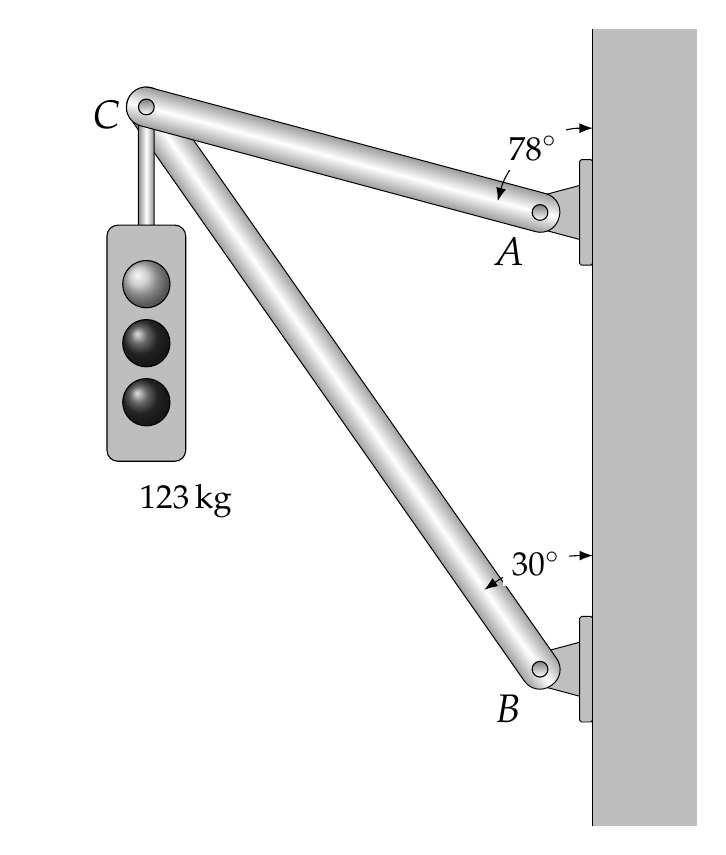
\begin{tikzpicture}

	\coordinate (C) at (0,0);
	\coordinate (B) at ($ (C)+(-15:5.176) $);
	\coordinate (A) at ($ (C)+(-55:8.717) $);
	\coordinate (D) at ($ (C)+(0,-3) $);

	\gettikzxy{(A)}{\ax}{\ay}
  \gettikzxy{(B)}{\bx}{\by}
  \gettikzxy{(C)}{\cx}{\cy}

	\PC[90]{B}{Gray!50}{black}{0.67}{0.125}
	\PC[90]{A}{Gray!50}{black}{0.67}{0.125}

	\fill[Gray0] ($ (\bx+0.67cm, \cy+1cm) $) rectangle ($ (\ax+2cm, \ay-2cm) $);
	\draw[thin]  ($ (\bx+0.67cm, \cy+1cm) $) -- ($ (\bx+0.67cm, \ay-2cm) $);
	
	\Meme{C}{A}{Gray}{White}{black}{0.5}{0.24}{0.125}	
	\Meme{C}{D}{Gray}{White}{black}{0.2}{.1}{0.125}
	\Meme{C}{B}{Gray}{White}{black}{0.5}{0.24}{0.125}

	\filldraw[rounded corners, fill=Gray0] ($ (D)+(-0.5,-1.5) $) rectangle ($ (D)+(0.5,1.5) $);
	\shadedraw[ball color=gray!40!black] (D) circle (.3cm);
	\shadedraw[ball color=gray!50] ($(D)+(0,0.75)$) circle (.3cm);
	\shadedraw[ball color=gray!40!black] ($(D)+(0,-0.75)$) circle (.3cm);
	\node at ($ (D)-(-0.5,2) $) {\large $ 123\,$kg};

	\draw[Latex-Latex] ($ (B)+(-15:0.6936)+(0,1.25) $) arc (90:165:1.25) node[midway,fill=white] {\large $78\deg$};
	\draw[Latex-Latex] ($ (A)+(-55:1.168)+(0,2.4) $) arc (90:125:2.4) node[midway,fill=white] { \large$30\deg$};

	\small
	
	\shadedraw [draw=black] (B) circle (0.1cm) node[ xshift=-0.4cm, yshift=-0.5cm] {\Large$A$};
	\shadedraw [draw=black] (A) circle (0.1cm) node[ xshift=-0.4cm, yshift=-0.5cm] {\Large$B$};
	\shadedraw [draw=black] (C) circle (0.1cm) node[ xshift=-0.5cm, yshift=-0.1cm] {\Large$C$};

	\pgfresetboundingbox
	\draw[white] (\cx-1.5cm, \cy+1cm) rectangle (\ax+2cm, \ay-2cm);
	

\end{tikzpicture}


}		
	}
\end{textblock*}

\begin{textblock*}{3.5in}(1in,1.5in)
	\centering
	Convert the mass of the traffic lights into a force:
	$$ W = 123\,\text{kg} \times 9.81\,\mathrm{m/s^2} = 1206.6\,\text{N} $$

	Note: By default, draw $F_{AC}$ and $F_{BC}$ in tension.\parb
	\tikz{%color
		\coordinate (C) at (0,0);
		\node[above left] at (C) {$C$};
		\draw[very thick, -latex] (C) -- +(0,-2.25)node[below]{$1206.6\,$N};
		\draw[very thick, -latex] (C) -- +(-12:2)node[right]{$F_{AC}$};
		\draw[very thick, -latex] (C) -- +(-60:2.25)node[right]{$F_{BC}$};
		\draw[latex-latex] ($ (C)+(-12:1.5) $) arc (-12:-60:1.5) node[midway, fill=white, inner sep=1mm] {$48\deg$};
		\draw[latex-latex] ($ (C)+(-60:1.75) $) arc (-60:-90:1.75) node[midway, fill=white, inner sep=0.25mm] {\normalsize $30\deg$};
	}
	\begin{align*}
		\sum F_x &= F_{AC}\cos 12\deg + F_{BC}\cos 60\deg = 0 \\[0.25em]
		\Rightarrow F_{BC} &= -\frac{F_{AC}\cos 12\deg}{\cos 60\deg} \\[0.25em]
		&= -1.9563F_{AC}
	\end{align*}
\end{textblock*}

\begin{textblock*}{3.5in}(4.5in,3.125in)
	\begin{align*}
		\sum F_y &= F_{AC}\sin 12\deg + F_{BC}\sin 60\deg + 1206.6\,\text{N}= 0 \\[0.25em]
		\Rightarrow 0 &= F_{AC}\sin 12\deg + F_{BC}\sin 60\deg + 1206.6\,\text{N} \\[0.25em]		
		\Rightarrow 0 &= F_{AC}\sin 12\deg -1.9563F_{AC}\cd\sin 60\deg + 1206.6\,\text{N} \\[0.25em]		
		\Rightarrow 0 &= F_{AC}\left(\sin 12\deg -1.9563\cd\sin 60\deg\right) + 1206.6\,\text{N} \\[0.25em]		
		\Rightarrow 0 &= -1.4863F_{AC} + 1206.6\,\text{N} \\[0.25em]		
		\Rightarrow F_{AC} &= 811.81\,\text{N} \\[0.25em]		
		\Rightarrow F_{BC} &= -1.9563(811.81\,\text{N})  \\[0.25em]		
		\Rightarrow F_{BC} &= -1588.2\,\text{N}  \\[0.25em]		
	\end{align*}
\end{textblock*}

\begin{textblock*}{6.75in}(1in, 5.5in)
	\centering
	The force in $\bm{AC=811}\,$N (Tension). The force in $\bm{BC=1590}\,$N (Compression).
\end{textblock*}

\begin{textblock*}{3.5in}(1in,5.75in)
	\cbox{
		\underline{Exercise 3} \parm
		Determine the internal forces in members $AC$ and $BC$. Specify whether they are in tension or compression.

	}
\end{textblock*}
\begin{textblock*}{2.75in}(5.025in, 5.75in)
	\cbox{
		\centering
		
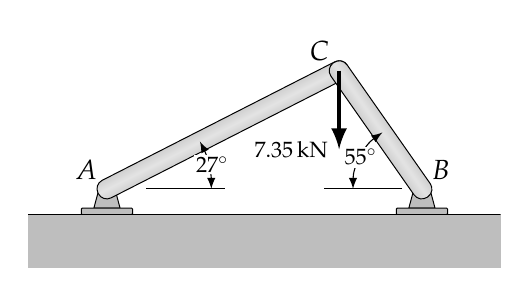
\begin{tikzpicture}

	\coordinate (A) at (-2,0);
	\coordinate (AA) at ($ (A)+(27:4) $);
	\coordinate (B) at (2,0);
	\coordinate (BB) at ($ (B)+(125:2.5) $);
	\path[name path=AC] (A)--(AA);
	\path[name path=BC] (B)--(BB);
	\path[name intersections = {of=AC and BC, by=C}];

	\PC{A}{Gray0}{black}{0.325}{0.125}
	\PC{B}{Gray0}{black}{0.325}{0.125}
	\fill[Gray0] ($ (A)+(-1,-0.325) $) rectangle ($ (B)+(1,-1) $);
	\draw ($ (A)+(-1,-0.325) $) rectangle ($ (B)+(1,-0.325) $);
	\Meme{A}{C}{LightGrey}{LightGrey!50}{black}{0.25}{0.12}{0.125}
	\Meme{B}{C}{LightGrey}{LightGrey!50}{black}{0.25}{0.12}{0.125}
	\draw[ultra thick, -latex] (C) -- +(0,-1) node[left]{\footnotesize $7.35\,$kN};
	\node[above left] at (C) {$ C $};
	\node[above left] at (A) {$ A $};
	\node[above right] at (B) {$ B $};

	\draw[thin] ($ (B)-(.25,0) $) -- +(-1,0);
	\draw[thin] ($ (A)+(.5,0) $) -- +(1,0);

	\draw[latex-latex] ($ (A)+(0:1.325) $) arc (0:27:1.325) node[midway, fill=white, inner sep=0.2mm, xshift=0.5mm] {\footnotesize $27\deg$};
	\draw[latex-latex] ($ (B)+(125:0.875) $) arc (125:180:0.875) node[midway, fill=white, inner sep=0.3mm] {\footnotesize $55\deg$};

	%  \Meme{A}{B}{Black}{White}{Red}{0.25}{0.125}{0.125}





	
	% \draw (current bounding box.south west) rectangle (current bounding box.north east);

	

\end{tikzpicture}


		
	}
\end{textblock*}

\begin{textblock*}{3.5in}(1in,7in)
	\centering
	\tikz{%color
		\coordinate (C) at (0,0);
		\draw[thick, -latex] (C)--+(0,-2)node[below]{$7.35\,\text{kN}$};
		\draw[thick, -latex] (C)--+(-55:2 )node[below]{$F_{BC}$};
		\draw[thick, -latex] (C)--+(207:2 )node[below]{$F_{AC}$};

		\node[above] at (C) {$C$};

		\draw[thin, gray] ($ (C)-(0.5,0) $) -- +(-1.25,0);
		\draw[thin, gray] ($ (C)+(0.325,0) $) -- +(1.25,0);

		\draw[latex-latex] ($ (C)+(0:1.25) $) arc (0:-55:1.25) node[fill=white, midway] {$55\deg$};
		\draw[latex-latex] ($ (C)+(180:1.5) $) arc (180:207:1.5) node[fill=white, midway, inner sep=0.2mm] {$27\deg$};
	}
	\begin{align*}
		\sum F_x &= F_{BC}\cos 55\deg - F_{AC}\cos 27\deg = 0 \\[0.25em]	
		\Rightarrow F_{AC} &= \frac{F_{BC}\cos 55\deg}{\cos 27\deg} = 0.64374F_{BC} \\\\
		\sum F_y &= F_{BC}\sin 55\deg + F_{AC}\sin 27\deg+ 7.35\,\text{N} = 0 \\[0.25em]
		&\Rightarrow  F_{BC}\sin 55\deg + (0.64374F_{BC})\sin 27\deg + 7.35\,\text{N} = 0 \\[0.25em]
		\Rightarrow F_{BC} &= \frac{-7.35\,\text{N}}{\sin 55\deg + 0.64374\sin 27\deg} = -6.6133\,\text{N} \\\\
		\Rightarrow  F_{AC} &= 0.64374(-6.6133\,\text{N}) = -4.2572\,\text{N}
	\end{align*}
\end{textblock*}

\begin{textblock*}{3in}(5.25in,8in)
	Or, setting up for the system-solver:
	\begin{align*}
		-\cos 27\deg\cd x + \cos 55\deg\cd y &= 0 \\
		\sin 27\deg\cd x + \sin 55\deg\cd y &= -7.35
	\end{align*} 
	\parb
	\raggedright
	The force in member $AC$ is 4.26\,\text{N} in compression and the force in member $BC$ is $6.61\,\text{N}$ in compression.
	
\end{textblock*}

%%%%%%%%%%%%%%%%%%%%%%%%%%%%%%%%%%%%%%%%%%%%%%%%%%%%%%%%%%%%%%%%%%%%%%%%%%%%%%%%%%%%%%%%%%%%%%%%%%%%
% page 3
%%%%%%%%%%%%%%%%%%%%%%%%%%%%%%%%%%%%%%%%%%%%%%%%%%%%%%%%%%%%%%%%%%%%%%%%%%%%%%%%%%%%%%%%%%%%%%%%%%%%
~\newpage

\begin{textblock*}{3in}(1in, 0.2in)
	\cbox{
		\underline{Example 4} \parm
		Determine $\theta$. Then find the tension in the rope and the pulley
		reaction at $B$ due to the suspended mass.
	}
\end{textblock*}
\begin{textblock*}{3.25in}(4.525in, 0.2in)
	\cbox{
		\centering
		\def\scale{0.8}
		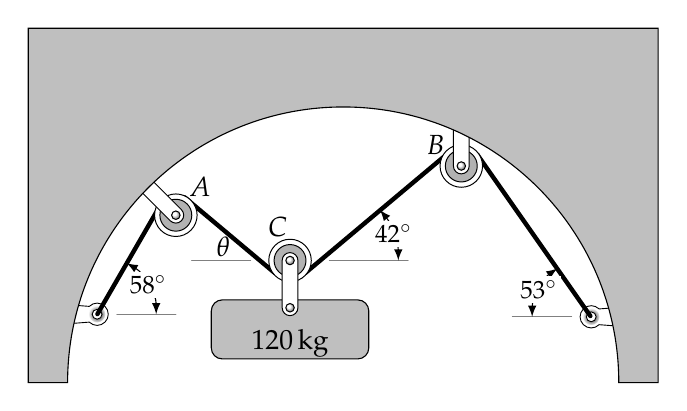
\begin{tikzpicture}[line cap=round]

  \coordinate (A) at (-2.125,2.125);
  \coordinate (B) at (1.5,2.75);
  \coordinate (C) at (-0.675,1.55);
  \coordinate (AA) at (-3.125,0.8675);
  \coordinate (BB) at (3.15,0.835);
  \coordinate (Cright) at ($ (C)+(0.375, 0) $);
  \coordinate (Cleft) at ($ (C)+(-0.375, 0) $);

 \filldraw[fill=Gray!50, rounded corners] ($ (C)+(-1,-.5) $) rectangle +(2,-0.75);
  \EyeBolt[-90]{AA}{White}{black}{0.5}{0.325}
  \EyeBolt[90]{BB}{White}{black}{0.5}{0.325}
  \draw[black, ultra thick] ($ (C)+(-40:0.25) $) -- +(40:2.3);
  \draw[black, ultra thick] ($ (C)+(220:0.25) $) -- +(140:1.5);
  \draw[black, ultra thick] ($ (A)+(170:0.25) $) -- +(240:1.5);
  \draw[black, ultra thick] ($ (B)+(35:0.25) $) -- +(-55:2.5);
  \PulleyC[225]{A}{White}{Black}{1.5}{0.25}{0.4}{0.125}
  \PulleyC[180]{B}{White}{Black}{1.5}{0.25}{0.4}{0.125}
  \PulleyC{C}{White}{Black}{1.5}{0.25}{0.4}{0.125}
  \filldraw[fill=Gray!50] (-4,0)-- +(0.5,0)arc(180:90:3.5)arc(90:0:3.5) -- (4,0) -- ++(0,4.5) -- ++(-8,0) -- cycle;
  \node at ($ (C)+(0,-0.75) $) [below] {$ 120\,$kg};
  \draw[thin, gray] ($ (C)+(0.5,0) $) -- +(1,0);
  \draw[thin, gray] ($ (C)+(-0.5,0) $) -- +(-0.75,0);
  \draw[thin, gray] ($ (BB)+(-0.25,0) $) -- +(-0.75,0);
  \draw[thin, gray] ($ (AA)+(0.25,0) $) -- +(0.75,0);
  \draw[latex-latex] ($ (Cright)+(1,0) $) arc (0:40:1) node[midway, fill=white, inner sep=0.5mm] {\small$42\deg$};
  \node at ($ (C)+(110:0.45) $) {$C$};
  \node at ($ (B)+(140:0.425) $) {$B$};
  \node at ($ (A)+(50:0.475) $) {$A$};
  \node at ($ (Cleft)+(160:0.5) $) {$\theta$};
  \draw[latex-latex] ($ (AA)+(0.75,0) $) arc (0:60:0.75) node[midway, fill=white, inner sep=0.5mm] {\small$58\deg$};
  \draw[latex-latex] ($ (BB)-(0.75,0) $) arc (180:125:0.75) node[midway, fill=white, inner sep=0.5mm] {\small$53\deg$};

  % \fill[green] (Cright) circle (0.5mm);


\end{tikzpicture}
	}
\end{textblock*}

\begin{textblock*}{3.5in}(1in, 1.75in)
	\centering
	\tikz{%color
		\coordinate (C) at (0,0);
		\draw[thick, -latex] (C) -- +(42:2) node[right] {$T$};
		\draw[thick, -latex] (C) -- +(138:2) node[left] {$T$};
		\draw[thick, -latex] (C) -- +(270:1) node[right] {$1177.2\,\text{N}$};
		\draw[thin, gray] ($ (C)+(0.4,0) $) -- +(1.5,0);
		\draw[thin, gray] ($ (C)+(-0.4,0) $) -- +(-1.5,0);
		\draw[latex-latex] ($ (C)+(1.5,0) $) arc (0:42:1.5) node[midway, fill=white] {$42\deg$};
		\draw[latex-latex] ($ (C)+(-1.5,0) $) arc (-180:-222:1.5) node[midway, fill=white] {$\theta$};
		\node[above,yshift=0.5mm] at (C) {$C$};
	}
	\begin{align*}
		\sum F_x &= T\cos 42\deg - T\cos\theta = 0 \\[0.25em]
		\Rightarrow \cos 42\deg &= \cos\theta \\[0.25em]
		\Rightarrow \theta &= 42\deg
	\end{align*}
	Note that pulley $C$ finds equilibrium when the angles of the cable on either side are equal.
	\begin{align*}
		\sum F_y &= 2T\sin 42\deg - 1177.2\,\text{N} = 0 \\[0.25em]
		\Rightarrow T &= \frac{1177.2\,\text{N}}{2\sin 42\deg} = 879.65\,\text{N} \\[0.25em]
	\end{align*}
	\tikz{%color
		\coordinate (B) at (0,0);
		\draw[red, ultra thick, -latex] (B) -- +(0,2) node[right] {$R_{By}$};
		\draw[red, ultra thick, -latex] (B) -- +(2,0) node[right] {$R_{Bx}$};
		\draw[thick, -latex] (B) -- +(-53:2) node[right] {$T$};
		\draw[thick, -latex] (B) -- +(222:2) node[left] {$T$};
		\draw[thin, gray] ($ (B)-(0.2,0) $) -- +(-1.5,0);
		\draw[latex-latex] ($ (B)-(1.25,0) $) arc (180:222:1.25)node[midway, fill=white, inner sep=0.5mm] {$ 42\deg $};
		\draw[latex-latex] ($ (B)+(1.25,0) $) arc (0:-53:1.25)node[midway, fill=white, inner sep=0.5mm] {$ 53\deg $};
		\node[above right] at (B) {$B$};
	}
\end{textblock*}

\begin{textblock*}{3.5in}(4.75in,2.75in)
	\begin{align*}
		\sum F_x &= R_{Bx}+ T\cos 53\deg -T\cos 42\deg = 0 \\[0.25em]
		\Rightarrow R_{Bx} &= T(\cos 42\deg-\cos 53\deg) \\[0.25em]
		&= 124.32\,\text{N} \\\\
		\sum F_y &= R_{By}- T\sin 53\deg -T\sin 42\deg = 0 \\[0.25em]
		\Rightarrow R_{By} &= T(\sin 42\deg+\sin 53\deg) \\[0.25em]
		&= 1291.1\,\text{N} 
	\end{align*}
	\centering
	\tikz{%color
		\coordinate (B) at (0,0);
		\draw[red, very thick, -latex] (B) -- +(0,3) node[left, black] {$1291.1\,\text{N}$};
		\draw[red, very thick, -latex] (B) -- +(0.62,0) node[below, black] {$124.32\,\text{N}$};
		\node[left] at (B) {$B$};
		\draw[-latex, very thick] (B)-- +(0.62,3);
		\node[xshift=0.25cm,yshift=0.225cm] at (B) {$\theta$};
	}
	\begin{align*}
		R_B &= \sqrt{(124.32\,\text{N})^2+(1291.1\,\text{N})^2} \\[0.25em]
		 &= 1297.1\,\text{N} \\\\
		 R_\theta &= \tan^{-1}\left[\frac{1291.1}{124.32}\right] \\[0.25em]
		 &= 84.500\deg
	\end{align*}
\end{textblock*}
\begin{textblock*}{6.75in}(1in,8.5in)
	\cmini[0.6]{
		\centering
		\large
		The tension in the cable is $880\,\text{N}$ \parb
		The reaction at $B$ is $1297.1\,\text{N}$ at $84.5\deg$, measured counter-clockwise from the positive $x$-axis.
	}
\end{textblock*}

`\newpage
\begin{textblock*}{3in}(1in, 0.2in)
	\cbox{
		\underline{Exercise 4} \parm
		Cylinder $B$ has a mass of 28 kg. The system is in equilibrium.
		Determine the mass of $A$ and the reactions at $C$ and $E$.

	}
\end{textblock*}
\begin{textblock*}{3.25in}(4.525in, 0.2in)
	\cbox{
		\centering
		\def\scale{0.8}
		% !TEX root = ../../Beamer/03EquilibriumOfAParticle/03Equilibrium.tex

\tikz[line cap=round, scale=0.9]{
	\coordinate (A) at (0,-2);
	\coordinate (B) at (0,0);
	\coordinate (C) at (-3,0);
	\coordinate (D) at ($ (30:3.746)+(-60:0.25) $);
	\coordinate (E) at ($ (D)+(0.2625,0)+(0,-2.5) $);

	\fill[right color=Gray, left color=Gray!50] ($ (C)+(-0.5,-1.5) $) rectangle +(-0.75,3);
	\fill[bottom color=Gray, top color=Gray!50] ($ (D)+(-1.5,.5) $) rectangle +(3,0.75);

	\EyeConnection[-90]{C}{Gray!50}{black}{0.5}{0.5}
	\Ring{B}{Gray!50}{Gray}{.25}{0.125}{0.01};

	\draw[ultra thick, Black] ($ (B)+(30:0.1) $) -- ++(30:3.646)arc(120:0:0.25)-- ++(0,-2.5);
	\draw[ultra thick, Black]($ (B)+(180:0.1) $) -- ($ (C)+(0.025,0) $);
	\draw[ultra thick, Black]($ (B)+(270:0.1) $) -- ++(0,-2);
	\Pulley[180]{D}{Gray0}{black}{0.5}{0.125}
	\draw[left color=Gray, right color=Gray, middle color=Gray!30] ($(A)+(-0.5,-.75)$) rectangle ($(A)+(0.5,0.75)$);
	\draw[left color=Gray, right color=Gray, middle color=Gray!30] ($(E)+(-0.5,-.75)$) rectangle ($(E)+(0.5,0.75)$);
	\draw[thin] ($ (B)+(0.5,0) $) -- +(1.5,0)node[right]{$ x $};
	\draw[latex-latex] ($ (B)+(1.5,0) $)arc(0:30:1.5)node[midway, fill=white, inner sep=0.25mm]{$ 32^\circ $};
	\node at (A) {\Large $A$};
	\node at (E) {\Large $B$};
	\node[yshift=0.5cm] at (C) {\Large $C$};
	\node[xshift=0.5cm] at (D) {\Large $E$};
	\node[xshift=-0.325cm, yshift=0.325cm] at (B) {\Large $D$};
	\node[ yshift=-1cm] at (E) {\large $28\,\text{kg}$};
}

	}
\end{textblock*}
\begin{textblock*}{3.5in}(1in, 1.5in)
	\centering
	$$ T_{DEB} = 28\,\text{kg}\times 9.81\,\mathrm{m/s^2} = 274.68\,\text{N} $$
	\tikz{%color
		\coordinate (D) at (0,0);
		\draw[thick, -latex] (D) -- +(32:2)node[right] {$274.68\,\text{N}$};
		\draw[thick, -latex] (D) -- +(180:1.5)node[left] {$T_C$};
		\draw[thick, -latex] (D) -- +(270:1.5)node[left] {$W$};
		\draw[thin, gray] ($ (D)+(0.5,0) $) -- +(1.25,0);
		\draw[latex-latex] ($ (D)+(1.5,0) $) arc (0:32:1.5) node [midway, fill=white] {$32\deg$};
		\node[above] at (D) {$D$};
	}
	\begin{align*}
		\sum F_x &= (274.68\,\text{N})\cos 32\deg-T_{CD} = 0 \\[0.25em]
		\Rightarrow T_{CD} &= 232.94\,\text{N} \\\\
		\sum F_y &= (274.68\,\text{N})\sin 32\deg-W = 0 \\[0.25em]
		\Rightarrow W &= 145.56\,\text{N} \\\\
	\end{align*}
	Cylinder $A$ has a weight of $145.56\,\text{N}$ so it has mass:$$A=\frac{145.56\,\text{N}}{9.81\,\mathrm{m/s^2}} = 14.838\,\text{kg}$$
	\parb
	\tikz{%color
		\coordinate (C) at (0,0);
		\draw[thick, -latex] (C)--+(2,0) node[below] {$ 232.94\,\text{N} $};
		\draw[thick, red, -latex] ($ (C)+(0,0.2) $) --+(1,0) node[above] {$ R_{Cx} $};
		\draw[thick, red, -latex] ($ (C)+(0,0.2) $) --+(0,1) node[right] {$ R_{Cy} $};
		% \node[xshift=0.75cm,yshift=0.225cm] at (D) {$\theta$};
		\node[left] at (C) {$ C $};
	}
	\parb
	\begin{align*}
		\sum F_x &= 232.94\,\text{N}+R_{Cx} = 0 \\[0.25em]
		\Rightarrow R_{Cx} &= -232.94\,\text{N}\\\\
		\sum F_y &= R_{Cy} = 0 
	\end{align*}
	\parb
	The reaction at $C$ is in the direction of the negative $x$-axis ($180\deg$ counter-clockwise from the positive $x$-axis.
\end{textblock*}

\begin{textblock*}{3in}(5in,3in)
	\centering
	\tikz{%color
		\coordinate (E) at (0,0);
		\draw[thick, red, -latex] (D) --+(1.5,0) node[above] {$ R_{Dx} $};
		\draw[thick, red, -latex] (D) --+(0,1.5) node[right] {$ R_{Dy} $};
		\draw[thick, -latex] (E) -- +(270:1.75)node[right] {$274.68\,\text{N}$};
		\draw[thick, -latex] (E) -- +(212:1.75)node[left] {$274.68\,\text{N}$};
		\draw[latex-latex] ($ (E)+(-90:1.25) $) arc (-90:-148:1.25) node [midway, fill=white, inner sep=0.5mm] {$58\deg$};
		\node[above left] at (D) {$D$};
	}
	\begin{align*}
		\sum F_x &= R_{Dx} -( 274.68\,\text{N})\sin 58\deg = 0 \\[0.25em]
		\Ra R_{Dx} &= 232.94\,\text{N} \\\\
		\sum F_y &= R_{Dy} -( 274.68\,\text{N})\cos 58\deg - ( 274.68\,\text{N}) = 0 \\[0.25em]
		\Ra R_{Dy} &= 420.24\,\text{N} 
	\end{align*}
	\parb
	\tikz{%color
		\coordinate (D) at (0,0);
		\draw[thick, red, -latex] (D) --+(1.2,0) node[black, below] {$ 232.94\,\text{N} $};
		\draw[thick, red, -latex] (D) --+(0,2.1) node[black,left] {$ 420.24\,\text{N} $};
		\draw[thick, -latex] (D) --+(1.2,2.1) node[right] {$ R_D $};
		\node[xshift=0.325cm,yshift=0.225cm] at (D) {$\theta$};
		\node[left] at (D) {$D$};
	}
	\parb
	\begin{align*}
		R_D &= \sqrt{(420.24\,\text{N})^2+(232.94\,\text{N})^2} \\[0.25em]
		 &= 480.48\,\text{N} \\\\
		\theta &= \tan^{-1}\left[\frac{420.24\,\text{N}}{232.94\,\text{N}}\right] \\[0.25em]
		&= 61.000\deg
	\end{align*}
\end{textblock*}

\begin{textblock*}{5.5in}(2in, 9.5in)
	\centering
	The mass of $A$ is $14.8\,$kg \parm
	The reaction at $C$ is $233\,\text{N}$ at $180\deg$, counter-clockwise from the positive $x$-axis.\parm
	The reaction $D$ is $480\,\text{N}$ at $61\deg$, counter-clockwise from the positive $x$-axis.
\end{textblock*}




%%%%%%%%%%%%%%%%%%%%%%%%%%%%%%%%%%%%%%%%%%%%%%%%%%%%%%%%%%%%%%%%%%%%%%%%%%%%%%%%%%%%%%%%%%%%%%%%%%%%
% page 6
%%%%%%%%%%%%%%%%%%%%%%%%%%%%%%%%%%%%%%%%%%%%%%%%%%%%%%%%%%%%%%%%%%%%%%%%%%%%%%%%%%%%%%%%%%%%%%%%%%%%
~\newpage


\begin{textblock*}{3in}(1in, 0.2in)
	\cbox{
		\underline{Example 5} \parm
		Determine the maximum weight $W$ of the bucket that the system can support given that no single wire may support more than $450\,$N. Determine $R_C$, the reaction at $C$, for this value of $W$.

	}
\end{textblock*}
\begin{textblock*}{3.25in}(4.525in, 0.2in)
	\cbox{
		\centering
		\def\scale{0.8}
		% !TEX root = ../../Beamer/03EquilibriumOfAParticle/03Equilibrium.tex

\tikz[line cap=round, scale=\scale]{
	\coordinate (A) at (0,0);
	\coordinate (B) at (2,0);
	\coordinate (C) at (6,2);
	\coordinate (D) at (4,-2);
	\coordinate (E) at (4,-3.5);





  \Ring{B}{LightGrey}{LightGrey}{0.25}{0.125}{0.02}
  \Ring{D}{LightGrey}{LightGrey}{0.25}{0.125}{0.02}

  \EyeConnection[-90]{A}{LightGrey!50}{black}{0.75}{0.5}
  \EyeConnection[90]{C}{LightGrey!50}{black}{0.75}{0.5}

  \draw[ultra thick, Black] ($(B)+(0.05,-0.05)$) -- ($(D)+(-0.05,0.05)$);
  \draw[ultra thick, Black] ($(A)+(0.05,0)$) -- ($(B)+(-0.0875,0)$);
  \draw[ultra thick, Black] ($(B)+(30:0.05)$) -- ($(C)+(210:0.05)$);
  \draw[ultra thick, Black] ($(D)+(63:0.05)$) -- ($(C)+(243:0.05)$);
  \draw[ultra thick, Black] ($(D)+(0,-0.05)$) -- +(0,-1);

	\filldraw[left color=LightGrey, right color=LightGrey, middle color=LightGrey!5] (E)-- ++(-0.5,0)-- ++(0.25,-1)-- ++(0.5,0)-- ++(0.25,1) -- cycle;

	\draw[thick] ($(E)+(0.5,0)$)arc(0:180:0.5);

  \fill[left color=LightGrey!40, right color=LightGrey] ($(A)+(-0.25,1)$) rectangle ($(A)+(-1,-2)$);
	\draw ($(A)+(-0.25,1)$) rectangle ($(A)+(-0.25,-2)$);
  \fill[right color=LightGrey!40, left color=LightGrey] ($(C)+(0.25,1)$) rectangle ($(C)+(1,-2)$);
	\draw ($(C)+(0.25,1)$) rectangle ($(C)+(0.25,-2)$);

  \node[below right] at (A) {$A$};
  \node[xshift=-0.325cm, yshift=0.325cm] at (B) {$B$};
  \node[xshift=-0.325cm,yshift=0.325cm] at (C) {$C$};
  \node[xshift=-0.325cm,yshift=-0.325cm] at (D) {$D$};
  \node[yshift=-0.5cm] at (E) {$W$};

  \draw[thin] ($(B)+(0.5,0)$) -- +(2,0);
  \draw[thin] ($(D)+(0.5,0)$) -- +(2,0);

\small
  \draw[latex-latex] ($(B)+(2,0)$)arc(0:26.565:2)node[midway, fill=white, inner sep=0.5mm]{$25^\circ$};
  \draw[latex-latex] ($(B)+(2,0)$)arc(0:-45:2)node[midway, fill=white, outer sep=1mm]{$45^\circ$};
  \draw[latex-latex] ($(D)+(1.5,0)$)arc(0:63.46:1.5)node[midway, fill=white, outer sep=1mm]{$60^\circ$};

}

	}
\end{textblock*}

\begin{textblock*}{4in}(0.5in,2in)
	\centering
	\tikz{
		\coordinate (O) at (0,0);
		\draw[-latex, thick] (O)-- +(0,-1)node[below]{$W$};
		\draw[-latex, thick] (O)-- +(65:2)node[left]{$F_{CD}$};
		\draw[-latex, thick] (O)-- +(135:2)node[left]{$F_{BD}$};
		\draw[thin] ($(O)+(0.5,0)$)-- +(1.5,0);
		\draw[thin] ($(O)+(-0.5,0)$)-- +(-1.5,0);
		\draw[latex-latex] ($(O)+(-1.5,0)$)arc(180:135:1.5)node[fill=white, midway]{$45^\circ$};
		\draw[latex-latex] ($(O)+(1.5,0)$)arc(0:65:1.5)node[fill=white, midway]{$60^\circ$};
		\node[below right] at (O) {$D$};
	}
	\begin{align*}
		\sum F_x &= F_{CD}\cos 60\deg - F_{BD}\cos 45\deg =0 \\[0.25em]
		\Ra F_{CD} &= \frac{F_{BD}\cos 45\deg}{\cos 60\deg}= 1.4142F_{BD}\\\\
		\sum F_y &= F_{CD}\sin 60\deg + F_{BD}\sin 45\deg-W =0 \\[0.25em]
		\Ra W &= F_{CD}\sin 60\deg + F_{BD}\sin 45\deg \\[0.25em]
		&= 1.4142F_{BD}\sin 60\deg + F_{BD}\sin 45\deg \\[0.25em]
		&= 1.9318F_{BD} \\[0.25em]
		\Ra F_{BD} &= 0.51764W \\[0.25em]
		\Ra F_{CD} &= 0.73205W
	\end{align*}
	\tikz{
		\coordinate (B) at (0,0);
		\draw[-latex, thick] (B)-- +(-2,0)node[left]{$F_{AB}$};
		\draw[-latex, thick] (B)-- +(30:2)node[right]{$F_{BC}$};
		\draw[-latex, thick] (B)-- +(-45:2)node[below]{$0.51764W$};
		\draw[thin] ($(B)+(0.5,0)$)-- +(1.5,0);
		\node[above left] at (B) {$B$};
		\draw[latex-latex] ($(B)+(1.5,0)$)arc(0:30:1.5)node[fill=white, midway, inner sep=0.5mm]{$25^\circ$};
		\draw[latex-latex] ($(B)+(1.5,0)$)arc(0:-45:1.5)node[fill=white, midway]{$45^\circ$};
	}
	\parm 
	\begin{align*}
		\sum F_y &= F_{BC}\sin 25\deg - 0.51764W\cd\sin 45\deg =0 \\[0.25em]
		\Ra F_{BC} &= \frac{0.51764W\cd\sin 45\deg}{\sin 25\deg} = 0.86609W \\\\
		\sum F_x &= (0.86609W)\cos 25\deg + 0.51764W\cd\cos 45\deg-F_{AB} =0 \\[0.25em]
		\Ra F_{AB} &= 1.1510W
	\end{align*}
	\parb
	\raggedright
	Comparing the tension values for all four cables, then highest tension is in cable $AB$. Set this tension to $450\,\text{N}$.
	\begin{align*}
		1.1510W &= 450\,\text{N} \\[0.25cm]
		\Ra W &= \frac{450\,\text{N}}{1.1510}= 390.96\,\text{N}
	\end{align*}
	
\end{textblock*}

\begin{textblock*}{3.75in}(4.625in,3.25in)
	\begin{align*}
		\text{Then, } F_{BC} & = 0.86609\times 390.96 = 338.61\text{ N} \\
		\text{and } F_{CD}   & = 0.73205\times 390.96 = 286.20\text{ N}
	\end{align*}
	\centering
	\tikz{
		\coordinate (C) at (0,0);
		\draw[-latex, thick] (C)-- +(240:2.5)node[below]{$286.20$ N};
		\draw[-latex, thick] (C)-- +(210:2.5)node[left]{$338.61$ N};
		\draw[-latex, very thick, red] (C)-- +(0,2)node[right]{$R_{Cy}$};
		\draw[-latex, very thick, red] (C)-- +(2,0)node[right]{$R_{Cx}$};
		% \draw[thin] ($(O)+(0.5,0)$)-- +(1.5,0);
		\draw[thin] ($(C)+(-0.5,0)$)-- +(-1.5,0);
		\draw[latex-latex] ($(O)+(-1.75,0)$)arc(180:210:1.75)node[fill=white, midway, inner sep=0.5mm]{$25^\circ$};
		\draw[latex-latex] ($(O)+(210:1.75)$)arc(210:240:1.75)node[fill=white, midway, inner sep=0.5mm]{$35^\circ$};
		\node[below right] at (C) {$C$};
	}
	\parb
	\begin{align*}
		\sum F_x      & = R_{Cx}-(338.61\,\text{N})\cos 25^\circ-(286.20\,\text{N})\cos 60^\circ =0           \\
		\Rightarrow R_{Cx} & = 449.98\,\text{N}                                          \\\\
		\sum F_y      & = R_{Cy} -(338.61\,\text{N})\sin 25^\circ-(286.20\,\text{N})\sin 60^\circ =0           \\
		\Rightarrow R_{Cy} & = 390.96\text{ N}                                          \\\\
		\Rightarrow R_C & = \sqrt{449.98^2+390.96^2}=596.10 \text{ N}                \\\\
		\theta          & = \tan^{-1}\left[\frac{390.96}{449.98}\right]=40.985^\circ
	\end{align*}
	\parb\large
	Maximum value for $W$ is $390\,\text{N}$ \parb
	Reaction at $C$ is $596$ N at $41.0^\circ$ ccw from the +ve $x$ axis.
	\parb
	\normalsize
	(Discussion: Should we round $390.96$ up to $391$ as we would normally do? Or not, because this pushes the tension in $AB$ marginally over $450\,\text{N}$?)
\end{textblock*}





%%%%%%%%%%%%%%%%%%%%%%%%%%%%%%%%%%%%%%%%%%%%%%%%%%%%%%%%%%%%%%%%%%%%%%%%%%%%%%%%%%%%%%%%%%%%%%%%%%%%
% page 7
%%%%%%%%%%%%%%%%%%%%%%%%%%%%%%%%%%%%%%%%%%%%%%%%%%%%%%%%%%%%%%%%%%%%%%%%%%%%%%%%%%%%%%%%%%%%%%%%%%%%
.\newpage

\begin{textblock*}{3.1275in}(1in, 0.225in)
	\cbox{
		\underline{Exercise 5} \parm
		The tension in cable $AC$ is $400\,$N. Determine the force $F$ necessary to hold the ring $A$ in the position shown..

	}
\end{textblock*}
\begin{textblock*}{3.125in}(4.65in, 0.225in)
	
	\cbox{
		\centering
		\def\scale{0.7}		
		% !TEX root = ../../Beamer/03EquilibriumOfAParticle/03Equilibrium.tex

\tikz[line cap=round, scale=\scale]{
	\coordinate (A) at (0,0);
	\coordinate (B) at (-3,3.5);
	\coordinate (C) at (4,3.5);
	\coordinate (D) at ($(A)+(0,-2)$);
	\coordinate (E) at ($(B)+(-0.275,-0.275)$);





	\Ring{A}{LightGrey}{LightGrey}{0.325}{0.1625}{0.02}
	\EyeConnection[180]{C}{LightGrey}{black}{0.75}{0.5}

	\draw[-latex, ultra thick] ($(A)+(130.6:0.1)$) -- ($(B)+(-49.4:0.05)$)arc(41.8:135:0.4)-- +(-1.25,-1.5)node[black, below]{$F$};
	\draw[ultra thick] ($(A)+(41.2:0.1)$) -- ($(C)+(221.2:0.05)$);
	\draw[-latex, ultra thick] ($(A)+(-90:0.1)$) -- +(-75:2.75)node[black, below]{$900$ N};

	\Pulley[180]{E}{LightGrey}{black}{0.75}{0.175}


	% 	\filldraw[left color=saitMaroon, right color=saitMaroon, middle color=saitMaroon!5] (E)-- ++(-0.5,0)-- ++(0.25,-1)-- ++(0.5,0)-- ++(0.25,1) -- cycle;
	%
	% 	\draw[thick] ($(E)+(0.5,0)$)arc(0:180:0.5);
	%
	\fill[LightGrey] ($(E)+(-2,0.75)$) rectangle +(4,1);
	\fill[LightGrey] ($(C)+(-2,0.75)$) rectangle +(4,1);
	\draw ($(E)+(-2,0.75)$) -- +(4,0);
	\draw ($(C)+(-2,0.75)$) -- +(4,0);

	\node[yshift=0.375cm] at (A) {$A$};
	\node[xshift=-0.1cm,yshift=-0.45cm] at (E) {$B$};
	\node[xshift=0.1cm,yshift=-0.35cm] at (C) {$C$};
	%
	\draw[thin] ($(A)+(0.5,0)$) -- +(2,0);
	% \draw[thin] ($(A)+(-0.5,0)$) -- +(-2,0);
	%
	\small
	\draw[latex-latex] ($(A)+(2,0)$)arc(0:-75:2)node[midway, fill=white, inner sep=0.5mm]{$75^\circ$};
	\draw[latex-latex] ($(A)+(2,0)$)arc(0:41.2:2)node[midway, fill=white, inner sep=0.5mm]{$41^\circ$};
	% \draw[latex-latex] ($(A)+(130.6:2)$)arc(130.6:180:2)node[midway, fill=white, inner sep=0.5mm]{$\theta$};

}

	}
\end{textblock*}

\begin{textblock*}{3in}(1in, 2in)
	\centering
	\tikz{
	\coordinate (A) at (0,0);
	\draw[-latex, thick] (A)-- +(41:2.5)node[above]{$400$ N};
	\draw[-latex, thick] (A)-- +(-75:2.5)node[below]{$900$ N};
	\draw[-latex, thick] (A)-- +(132:2.5)node[left]{$F$};
	\draw[thin] ($(A)+(0.5,0)$)-- +(1.5,0);
	\draw[thin] ($(A)+(-0.5,0)$)-- +(-1.5,0);
	\draw[latex-latex] ($(O)+(-1.5,0)$)arc(180:132:1.5)node[fill=white, midway, inner sep=0.5mm]{$\theta$};
	\draw[latex-latex] ($(O)+(0.5:1.5)$)arc(0:41:1.5)node[fill=white, midway, inner sep=0.5mm]{$41^\circ$};
	\draw[latex-latex] ($(O)+(0.5:1.5)$)arc(0:-75:1.5)node[fill=white, midway, inner sep=0.5mm]{$75^\circ$};
	\node[below left] at (A) {$A$};
	}
	\parb
	\begin{align*}
		\Sigma F_x &= 400\,\text{N}\cd\cos 41^\circ + 900\,\text{N}\cd\cos 75^\circ-F\cos\theta=0\\
		\Rightarrow F\cos\theta &= 534.82\text{ N}\\\\
		\Sigma F_y &= 400\,\text{N}\cd\sin 41^\circ - 900\,\text{N}\cd\sin 75^\circ+F\sin\theta=0\\
		\Rightarrow F\sin\theta &= 606.91\text{ N}\\\\
		\theta &= \tan^{-1}\left[\frac{F\sin\theta}{F\cos\theta}\right]=\tan^{-1}\left[\frac{606.91}{534.82}\right]=48.613^\circ\\\\
		F &= \frac{606.91\text{ N}}{\sin 48.613^\circ} = 808.93\text{ N}
	\end{align*}
	\parb

	$F=809\,\text{N}$ and $\theta=48.6\deg$
\end{textblock*}

\end{document}